\documentclass{llncs}

\usepackage{graphicx}

\title{Workflows and Distributed Version Contro}
\author{Olof Johansson \and Daniel Persson}
\institute{Blekinge Institute of Technology}

\begin{document}

\maketitle

\begin{abstract}
 This is a bachelor thesis in software engineering on Blekinge
 Institute of Technology, investigating version control systems
 in relation to software development in general and VCS related
 workflows in particular. Specifically, we investigate
 \emph{distributed} VCS. We also try to investigate the
 relationship between VCS workflows and code quality.
\end{abstract}

\section{Introduction}

As part of a software engineering project at Blekinge Institute of
Technology, the authors are investigating the use of version control
systems (VCS), specifically distributed VCS (DVCS), in the context of
the project (through a post-mortem analysis (data collections, 
interviews and observations)) and more generally through the use of a
literature review. The paper will try to answer the following questions:

\begin{itemize}
 \item How do the developers adapt to a distributed workflow?
 \item How does a distributed workflow affect code quality in relation
       to the release management and code review?
\end{itemize}

The primary means of doing the post-mortem analysis will be
to conduct interviews with participants in their various roles. In
addition to this we will also collect data from various project
management and configuration management tools and systems.

\section{Background}

The history of Version Control Systems can be divided into three
categories; the ones that only manages local files, the ones that rely
on a central server to serve connecting clients, and finally the
distributed ones, where every 'node' can act as both a client and a
server. The three categories roughly follow each other
chronologically, naturally with transition-periods in between. At the
moment the dominating tools are mostly client-server, but the
distributed ones are rising fast in popularity, so perhaps we are
currently in the start of a new transition.

\subsection{The Local Era}
The first VCS ever released was the \emph{Source Code Control System}
(SCCS) in 1972. SCCS tried to solve a number of problems that software
developers of that time had. Manually managing several versions of the
same product simultaneously was not feasible in the long run for
several reasons described by the creator of SCCS, Marc J. Rochkind
\cite{rochkind75}:

\begin{itemize}
 \item The amount of space to store the source code may be several
       times that needed for any particular version.
 \item Fixes made to one version sometimes fail to get made to
       other versions.
 \item When changes occur it is difficult to tell exactly what changed
       and when.
 \item When a customer has a problem it is hard to figure out what
       version he has.
\end{itemize}

Instead of saving entire files in various states, SCCS stores the
differences between versions of the same file (called diffs, or
deltas). With each delta SCCS also stores metadata such as who made
the change, why, and when. This did not only save precious storage
space, but also provided the \emph{traceability} that the software
developers had previously lacked.

It is worth noting that SCCS was not the only VCS that followed the
philosophy of storing the files locally, \emph{Revision Control
System} (RCS) which was essentially a wrapper around the Unix tool
\emph{diff} was released in 1982 and gradually started taking over as
the dominant VCS for Unix.

\subsection{The Client-Server Era}
Although RCS was an improvement over SCCS it still had several flaws;
it was still operating on single files only, and they were still
stored locally. 

To be able to cooperate with his students, working on differing
schedules, Dick Grune created shell scripts to centrally manage the
project they were working on through RCS. When the project was over he
realized the potential and cleaned up the scripts and published them
in late 1985. Two years later Brian Berliner rewrote the software in
C, and CVS was born.

CVS introduced all the modern terminology we use today when we talk
about version control; the code is stored in a \emph{repository} that
users can \emph{check out} a \emph{working copy} from. Terms such as
\emph{committing} code and \emph{merging} changes was also introduced
by CVS. It also made \emph{branching} a bit less cumbersome than it
had been in RCS although merging the branches still required a lot of
work.

With CVS in the front line and with proprietary version control
systems starting to pop up in the early nineties the model of a
central server that contained the repository that everyone worked in
became the standard way to think about version control.

Although CVS simplified and popularized the use of version control
systems it has still received its fair share of criticism. For example
the revision numbers are created on a per file basis, which means that
the latest revision number is not the same across the board which can
sometimes be confusing. Other things like not handling symbolic links
for example is claimed by the CVS developers to be carefully planned
features (in the case of symbolic links due to security concerns)
rather than bugs, but as the issues started to pile up Collabnet
(founded by Tim O'Reilly that founded \emph{O'Reilly Media} and Brian
Behlendorf, co-founder of the Apache project) started the Subversion
project.

Subversion was released in 2000, and solved many of the issues that
CVS had, while still maintaining the same working style of
CVS. Subversion didn't really introduce any revolutionary ideas, but
rather focused on the weaknesses of CVS like versioning of symbolic
links, versioning for directories and file metadata and truly atomic
commits (meaning if the transmission between client and server is
interrupted, the commit is rolled back rather than processed half-way,
much like transaction in a database --- in CVS this wasn't the case,
and it could cause inconsistencies or corrupted data if it happened).

Other systems such as IBM's ClearCase and Microsoft's Visual
SourceSafe and Team Foundation Server existed, but never reached the
same popularity as CVS (that even to date manages a significant amount
of projects) and Subversion (that is currently the most popular tool
for version control) due to its proprietary licensing.

\subsection{The Distributed Era}

The next innovation came from the open source community, where the
centralized approach of CVS and Subversion didn't come as natural as
it perhaps does in the corporate domain. Instead of storing the
repository on a centralized server, distributed version control
systems like GNU Arch and Monotone stored a copy of the repository on
every client that checked out a working copy. That way developers
could always have access to the full history even without an internet
connection.

One of the first distributed version control systems, BitKeeper,
infamously withdrew the rights for the Linux kernel project to freely
use BitKeeper (which was a proprietary system) which sparked Linus
Torvalds to create a new, free tool: Git. 

The main goal with git was to create a version control system that
supported a BitKeeper-like workflow with high performance and strong
integrity control. Since Linus also has a passionate hatred for CVS he
has also said ironically that if there is any doubt in any design
choice to be made, the opposite of the one CVS took is the way to go.

Git has in the past few years seen a steady growth in users and
projects, and while the numbers compared to Subversion is still quite
small, the change speed is pointing straight up.

\subsection{VCS Workflow}

VCS can be used in a number of ways. Some limits are posed by the choice
of tools. Subversion is built for centralized version control, whereas
tools like git or mercurial are built for decentralized. Members of the 
latter category are generally more flexible; e.g. git is almost as simple 
to run centralized as running it decentralized as it is intended. The 
Telia Smart Home project has chosen to use git. The reasons for this are
several: the ability to use git decentralized as well a centralized was a
major point. Also, the prior experience from some members of the project
made the transition for other members less burdensome.

But defining a workflow does not end with selecting a tool. As stated, 
git is very flexible in the way developers interact with it. It is not
uncommon to use it centralized, and in fact, the Telia Smart Home project
does just this in their documentation repository. But one of the key 
strength is its decentralization. It has no enforced "central repository"
through which all changesets must pass. If the team want to have a 
centralized repository it must itself give a arbitrary repository that
semantic meaning.

Are there any alternatives to be considered? Certainly. Again, git is 
indeed quite flexible. It will yield to the wishes of the user. There are 
a number of easily recognized workflows (perhaps not always mutually
exclusive). Some of the most popular ones are presented here:

\begin{itemize}
 \item \textbf{Centralized}: 
  Using git in a way similar to e.g. Subversion or other more traditional
  tools still give the user some advantages. The process of branching and
  merging is many times more well developed in git than it is in tools like
  Subversion. A property of the distributed nature of git gives yet another
  benefit: having all of the history available locally. You don't need
  network to be able to see what changes was introduced to a particular
  commit, and indeed no network to be able to see the commit log.

 \item \textbf{Topic branches}: 
  Working on a new cool, but experimental feature? Perhaps it is not as 
  tested as the rest of the system is. You probably don't want to have 
  it in the main code. Create a branch specifically for this "topic" or
  "feature".

 \item \textbf{Benevolent dictator}: 
  A workflow, especially popular within open source projects, is the
  benevolent dictator workflow. There is one designated maintainer, and
  other contributers make "pull requests", primarily via e-mail.  If the
  benevolent dictator accepts the patch, he or she merges it into his or
  hers own repository, where everybody gets their source code from. The
  name, "Benevolent dictator", is a term jokingly used about Linus
  Torvalds, the initial author and later primary maintainer for the Linux
  kernel (and also, the initial author of git!).
\end{itemize}

\begin{figure}
 \begin{center}
  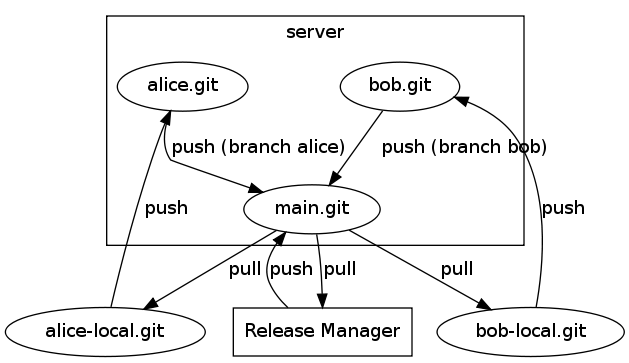
\includegraphics[scale=0.5]{workflow.png}
  \caption{Workflow description}
  \label{fig:workflow}
 \end{center}
\end{figure}

Each of these workflows are appropriate in some situations. However,
none of these totally fitted the needs of the Telia project. Instead,
the Telia Smart Home project designed its own workflow (see Figure
\ref{fig:workflow}). The workflow used for the code repositories in the
project is based upon individual developer repositories and branches.
Each developer has an own repository, and makes commits to this. The
system (with the help of so called hooks (i.e. scripts triggered by
specific events)) then pushes changes to a repository on a central build
server. Here, a build is triggered using the \emph{Jenkins} continuous
integration system and the commit is also forwarded to the so called
"baseline" repository, but only to a developer's private branch. It is
not merged into the actual baseline code, but it is still accessible for
other developers.

The release manager is now notified that there is a commit awaiting
approval. He or she can check build and test status on Jenkins and see the
delta between baseline and the proposed patch. After possibly running local
tests, the release manager can either approve and merge the commit or
reject it, and inform the author of why it wasn't suitable for inclusion.
If the commit is merged, other developers are now encouraged to merge it 
into their local repositories, their working copy of the source code. 

When designing this system, the sought benefits was the integrated code 
review and approval system. With this, the release managers could validate 
adherence to coding conventions as well as making sure that the system
is buildable and all unit tests passes. Possibly, much of this could even
have been automated (e.g. static code analysis and coding style validation
tools are commonplace) to an even higher degree, but that is, as always, a 
cost/benefit question. It is innovative and unique, but it does build upon
the so called "benevolent dictator" workflow, especially the release
management component of it. The success of this workflow from high-profile 
projects like the Linux kernel has been an inspiration for the design.
The reason why the project rejected the topic branch workflow at an early
stage was the problems associated with topic branches in the early stages
of a software project, where a lot of interdependencies exist and basic
infrastructure is needed. In later stages of the project, this workflow
would have been more feasible, but the overhead associated with switching
workflow was deemed to high. It has been used in some rare cases, where code
was at a very experimental stage.

\section{Literature Review}

%* in common

\subsection{Migration costs}

There a large number of open source as well as proprietary projects
moving to one of the major distributed version control system; Perl,
Curl and Parrot are projects that all has migrated to Git, from their
earlier centralized VCSes\footnote{
 Perl migrated from Perforce, Curl from CVS and Parrot from Subversion.
}. The migrations has not always been cheap, e.g. the Perl migration 
took 22 months \cite{alwis09}, so they must have had good reasons to 
do it. We will try to see why this might have been in the next few
subsections.

A migration of VCS is twofold. There is migration of the repository,
with moving every commit with its meta data and authorship
information, every branch and every tag to the new VCS, making sure
that nothing is lost and that nothing is broken. A problem in its own
right, but with a lot of tools available producing generally good
results. The other side, however, is migrating the developers and the
workflows. Changes in interface design requires every developer to
"relearn" the various actions and tools used. Something as trivial as
commit IDs are different and has become a problem for some
\cite{alwis09} --- the centralized VCSes commonly use incremental
integers to identify a commit; DVCSes usually use a checksum of the
content instead. The incrementing integers says more to a human when
comparing two commits, which of the two commits are the newest, and
perhaps gives a hint about how much newer \cite{bird09}. The loss is
an unfortunate effect of the distributed nature of DVCS. As every
repository is "isolated" from each other, and only interacts when
merging with each other, they can not know what numeric ID they should
give to a commit to make it globally unique and still retain the
incremental property.  So instead checksums are used; well known
algorithms are used to calculate a large value based on the contents
of the commit. This difference between DVCS and VCS is one of the
first a new DVCS user encounters.

Another change from centralized VCS is the decoupling of committing
and merging. This makes it a two command operation to do the
equivalent of "svn commit". Looking past the short term
impracticalities of having to do two commands to merge with a central
server, it gives the developer freedom to not merge at all, or not
merge "right now". Perhaps it is not even possible to merge --- as is
the case in airplanes or being in remote areas and no network
connectivity is available.

An other change, not a change in the interface but a change of VCS
nomenclature, is perhaps an even bigger obstacle for migration
\cite{bird09}. Some words are introduced, some words are removed and
some words are redefined. Committing is, as described, no longer
publishing your changes in the central repository. Pulling and pushing
are common words within DVCS for things that don't even exist in a
centralized VCS. In short, there will have to be a lot of
documentation of procedures, tools and workflows when migrating to a
new VCS --- especially a DVCS \cite{alwis09}.

\subsection{Architecture}

As mentioned in the section on migration costs, the fundamental
differences in the distributed version control architecture vis a vis 
the centralized ditto makes it hard to transfer workflows and
techniques directly. The differences do make it possible to other
things and brings number of benefits together with its disadvantages.

The distributed nature means that you have certain limitations on what
can be done to enforce synchronization: e.g. there is no file locking
support (making sure that only one developer works on a certain file
at a time) \cite{osullivan09} and it's harder to impose automated
content control. It makes it hard to delete history --- this would
have been problematic for e.g. the FreeBSD developers when they were
forced by a court decision to cease distribution of certain older
components \cite{alwis09}. But by the same token, it works as an
implicit distributed backup system, where each checked out repository
is a repository in its own right. Data loss at a single node won't be
a critical issue, as the complete repository with content and history
is replicated numerous times \cite{alwis09}. Another benefit from the
distributed architecture of DVCS is the ability to work independently,
isolated from the central repository. With this, a developer could
work when travelling to or from remote offices or conferences
\cite{alwis09}\cite{robert06}.

The research done in the field has largely depended on the activities
of various open source projects, with its wealth of openly accessible
data and discussions \cite{alwis09}\cite{bird09}. These kind of
projects has some specific problems and needs, some which only has a
limited effect on non open source projects. One positive effect of
distributed version control systems is that it lowers the bar for new
contributors. They can easily fork a project and commit changes, and
then make a request to be merged into the mainline \cite{alwis09}.
This limits the phenomenon known as "commit whoring" or "commit
politics", where people try to get commit access just for the sake of
it (as a status symbol).

\subsection{Performance}

The fact that anyone using a DVCS is working with a local repository
has big impacts on performance. In a CVCS every operation requires
access to the central server, and thus adds network latency to every
operation. Additionally, every developer that works towards the same
central server adds more to its workload, making it scale quite
badly. In contrast, DVCSes do not work towards the same server, even
though some repositories are perhaps considered 'more important' than
others, and thus scales very well almost any amount of
developers. Working locally leads to operations like branching and
merging being much faster and smoother, encouraging developers to use
them more\cite{alwis09}.

\subsection{Quality Implications}

The fact that most operations are so fast in DVCSes will have an
impact on how people work with their SCM tools. The fact that
branching is such a cheap operation will encourage developers to
actually use branches where they see fit, without taking things like
workload on a central server, namespace pollution, or wait times into
consideration. Coupled with the fact that merging branches is
relatively painless --- and thus resulting in merging being done when it
should, instead of being postponed to delay the suffering for the
developer, creating unnecessary conflicts and more suffering --- will
in turn lead to a more thorough and in a sense more correct use of the
VCS, resulting in a better history and potentially better code.

Another powerful tool that can be used more frequently due to the huge
performance-benefits that DVCSes provide is \verb!bisect!. It is very
easy to use, but can prove to be very useful in finding bugs, or
rather finding out when they are introduced. What \verb!bisect! does
is basically a binary search between two revisions (between which you
know that a bug is introduced) by checking out revisions and asking
the developer if the bug is present or not. Provided that the bug can
be replicated with for example a script, this task can be automated
fairly easy, and the fact that everything runs locally keeps the
performance up, and prevents the network from being congested.
Needless to say, when looking for a particular bug it is a huge
advantage to know the exact commit that introduced it.

Since the primary mean of sharing and spreading code in a DVCS
workflow is by pulling other peoples changes into a local repository,
introducing quality practices like \emph{code reviews} fits in very
well. Whenever anyone pull code from someone else, they simply look at
the diff, and if it does not meet the agreed upon quality standards,
they don't merge them until they do\cite{osullivan09}.

\section{Results from Post-mortem Analysis}

From the conducted interviews it is noticable that survey participants
rated their proficiency with DVCSes the same as with VCSes in general.

Regarding the workflow employed by the Telia Smart Home (TSH)
project, the survey conducted resulted in generally positive feedback,
with only some minor reservations. Some concern was raised regarding
the way the project ``abused git'' in the way branches were
automatically re-pushed to branches in the mainline
repository. A problem with the release manager approach was that it
easily becomes a bottleneck, if for example the release manager is
absent or busy. Several survey participants claimed to have
experienced this problem. Another survey participant noted that the
workflow looked more complex than it really was. Other participants
noted that the code review came natural and worked well, and that the
mainline build was rarely broken.

\section{Discussion}

The re-pushing of branches could very well have been excluded from the
workflow, the reasons for having it was to ease the work for release
managers by having all changes in one repository and not spread
out. The other reason was to allow easy overview in the issue tracking
system (Redmine) which was limited to only show one repository.

The release management criticism is not in any way limited to the TSH
workflow, it is present in any workflow using a review process to
accept and merge commits. One possible solution could be for example
having a dedicated person for the review process, but in this project
the cost would have been too big. Sharing the responsibility of
release management between several people could also remove the
downtime of the review process when the release manager is
absent. Overall the release management and code review has worked
well, with few hick-ups, and as figure \ref{fig:breakage} shows, the
mainline build was broken relatively few times, and only for short
periods of time.

\begin{figure}
 \begin{center}
  \caption{FIXME}
  \label{fig:breakage}
 \end{center}
\end{figure}

\section{Conclusion}

\bibliographystyle{plain} 
\bibliography{references}

\end{document}

